\scanpage{30}
% archive sheet number: 29
% Landscape sheet. Faint rotated, mirror-reversed typescript is verso show-through.
% Upper-left abandoned fragment.
\[\Delta X_n,\,\unsure{\deleted{-s}|\longleftarrow s}\]
\[
\langle\Delta X_n,s^p\otimes s^q\rangle=\langle X_n,s^{p+q}\rangle=\delta_{n,p+q}
\]
\[
\boxed{\left\{\begin{aligned}
\Delta X_n&=\sum_{p+q=n}X_p\otimes X_q\\
X_pX_q&=\sum_{\sup(p,q)\leq n\leq p+q}\frac{n!}{(n-p)!\,(n-q)!\,(p+q-n)!}X_n
\end{aligned}\right.}
\]
% Upper right, small note and calculation.
% TikZ ellipse decoration used for the circled pairing.
\usetikzlibrary{shapes.geometric}
\margin{$\Delta s=s\otimes1+1\otimes s\unsure{-|+}s\otimes s$}
\diagram{\begin{tikzcd}[ampersand replacement=\&,column sep=small,row sep=large]
\langle X_p.X_q,s^n\rangle=\&|[draw,ellipse]|\langle X_p\otimes X_q,(\Delta s)^n\rangle\arrow[d,leftrightarrow]\\
\deleted{\unsure{\delta}}\&
\left\{\begin{aligned}
0&\quad\text{si }\deleted{\unsure{n}}\ \unsure{\operatorname{Non}}(p,q\leq n\leq p+q)\\
\frac{n!}{(n-q)!\,(n-p)!\,(p+q-n)!}&\\[-2pt]
&\text{sinon}
\end{aligned}\right.
\end{tikzcd}}
\[
\sum_{\alpha+\beta+\gamma=n}\frac{n!}{\alpha!\,\beta!\,\gamma!}s^{\alpha+\gamma}\otimes s^{\beta+\gamma}
\qquad
\left\{\begin{aligned}
\alpha+\deleted{\unsure{\beta}}\gamma&=p\\
\beta+\gamma&=q
\end{aligned}\right.
\]
\[
\alpha+\beta+2\gamma=p+q\qquad
\left\{\begin{aligned}
\gamma&=p+q-n\\
\alpha&=n-q\\
\beta&=n-p
\end{aligned}\right.
\qquad p,q\leq n\leq p+q
\]
% Middle left.
\[
\left\{\begin{aligned}
\unsure{\delta|\Delta}X_n&=\sum_{\substack{p+q=n\\p,q>0}}X_p\otimes X_q
\end{aligned}\right.
\]
% Central tensor line, with a bracket under the inner terms.
\figure{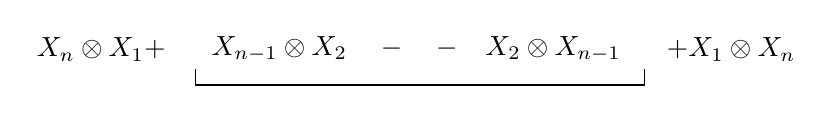
\begin{tikzpicture}
\node (a) at (0,0) {$X_n\otimes X_1+$};
\node (b) at (4.0,0) {$X_{n-1}\otimes X_2\quad-\quad-\quad X_2\otimes X_{n-1}$};
\node (c) at (8.0,0) {$+X_1\otimes X_n$};
\draw (1.2,-.25)--(1.2,-.45)--(6.9,-.45)--(6.9,-.25);
\end{tikzpicture}}
\[\unsure{U_n|\mathcal U_n|U_m|\mathcal U_m}\qquad\delta X_n\]
% Lower-right abandoned arrows, then live diagram.
\diagram{\begin{tikzcd}[ampersand replacement=\&]
\deleted{\unsure{\delta}}\&\deleted{U}\arrow[r]\&\deleted{U\otimes U}\arrow[r]\&\deleted{U}
\end{tikzcd}}
\diagram{\begin{tikzcd}[ampersand replacement=\&]
A\&A\otimes A\arrow[l]\&A\arrow[l]\\
G\arrow[r,"{\text{diag}}"']\&G\times G\arrow[r,"{\text{mult.}}"']\&G
\end{tikzcd}}
% Lower-left computation and continuation to its right.
\[X_2\]
\[X_1^2=2X_2+X_1\]
\[
\left\{\begin{aligned}
2X_2&=X_1^2-X_1\\
\delta X_2&=X_1\otimes X_1
\end{aligned}\right.
\qquad ?\qquad 2\delta X_2=\delta(X_1^2-X_1)
\]
\[\deleted{\unsure{2.\delta(X_1}}\]
\[2X_1\otimes X_1=\delta(X_1^2-X_1)\]
\[
\begin{aligned}
\delta(X_1)&=X_1\otimes1+1\otimes X_1\\
\delta(X_1^2)&=X_1^2\otimes1\unsure{-|+}1\otimes X_1^2+2X_1\otimes X_1
\end{aligned}
\]
